% Capítulo 3: lista duplamente encadeada.
\documentclass[border=4pt]{standalone}
\usepackage[utf8]{inputenc}
\usepackage[T1]{fontenc}
% Estilo comum das figuras de listas (incluído pelas figuras dos capítulos 3 e 4).
\usepackage{tikz}
\usetikzlibrary{arrows.meta, positioning, shapes.multipart, calc}
\definecolor{navy}{RGB}{23,45,80}
\definecolor{laranja}{RGB}{250,110,29}
\definecolor{cinzalogo}{RGB}{107,114,126}
\tikzset{
  no/.style={rectangle split, rectangle split horizontal, rectangle split parts=2,
             draw=navy, line width=0.9pt, minimum height=7mm,
             rectangle split part fill={laranja!15, white}, font=\sffamily\small},
  no3/.style={rectangle split, rectangle split horizontal, rectangle split parts=3,
              draw=navy, line width=0.9pt, minimum height=7mm,
              rectangle split part fill={white, laranja!15, white}, font=\sffamily\small},
  seta/.style={-{Stealth[length=2.2mm]}, navy, line width=0.9pt},
  setanova/.style={-{Stealth[length=2.2mm]}, laranja, line width=1.3pt},
  rotulo/.style={font=\sffamily\small\bfseries, text=navy},
  nulo/.style={font=\sffamily\scriptsize, text=cinzalogo},
  passo/.style={font=\sffamily\small, text=cinzalogo, anchor=west},
  legenda/.style={font=\sffamily\scriptsize, text=cinzalogo},
}
% seta que sai do meio da caixa do ponteiro (última parte do nó), na horizontal
\newcommand{\liga}[3][seta]{\draw[#1] ([xshift=-2.3mm]#2.east) -- #3;}

\begin{document}
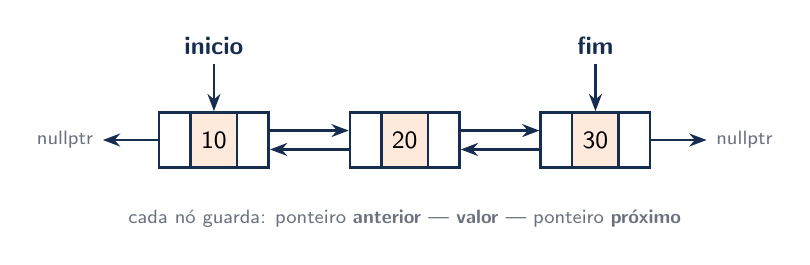
\begin{tikzpicture}[node distance=10mm]
  \node[no3] (a) at (0,0) {\phantom{x} \nodepart{two} 10 \nodepart{three} \phantom{x}};
  \node[no3, right=of a] (b) {\phantom{x} \nodepart{two} 20 \nodepart{three} \phantom{x}};
  \node[no3, right=of b] (c) {\phantom{x} \nodepart{two} 30 \nodepart{three} \phantom{x}};
  \node[nulo, left=7mm of a] (n0) {nullptr};
  \node[nulo, right=7mm of c] (n1) {nullptr};
  \node[rotulo, above=6mm of a] (ini) {inicio};
  \node[rotulo, above=6mm of c] (fim) {fim};
  \draw[seta] (ini) -- (a.north);
  \draw[seta] (fim) -- (c.north);
  \draw[seta] ([yshift=1.2mm]a.east) -- ([yshift=1.2mm]b.west);
  \draw[seta] ([yshift=-1.2mm]b.west) -- ([yshift=-1.2mm]a.east);
  \draw[seta] ([yshift=1.2mm]b.east) -- ([yshift=1.2mm]c.west);
  \draw[seta] ([yshift=-1.2mm]c.west) -- ([yshift=-1.2mm]b.east);
  \draw[seta] (a.west) -- (n0);
  \draw[seta] (c.east) -- (n1);
  \node[legenda, below=4mm of b] {cada nó guarda: ponteiro \textbf{anterior} | \textbf{valor} | ponteiro \textbf{próximo}};
\end{tikzpicture}
\end{document}
